\documentclass{book}

%%%%%% Import Package %%%%%%
\usepackage{graphicx}
\usepackage[unicode]{hyperref}
\usepackage{cite}
\usepackage{indentfirst}
\usepackage{multirow}
\usepackage{indentfirst}
\usepackage{titlesec}
\usepackage{xcolor}
\usepackage{listings}
\usepackage{fontspec,xunicode,xltxtra}
\usepackage{xeCJK}
\usepackage{hyperref}
\usepackage{enumerate}
\usepackage{epigraph}
\usepackage{amsmath}
\usepackage[xindy]{glossaries}
\usepackage{fancyhdr}
\usepackage{amsmath}
\usepackage{longtable}

%When compile under liunx% 
%\setmainfont{WenQuanYi Micro Hei}  
%\setmainfont{WenQuanYi Zen Hei Mono} 

\newcounter{coderemarks}   %创建变量
\setcounter{coderemarks}{1}   %设置变量初值为1
\newcounter{codevar}     %创建变量
\setcounter{codevar}{1}     %设置变量初值为

\newcommand{\circlemark}[1]{%
\tikz\node[text=white,font=\sffamily\bfseries,inner sep=0.2mm,draw,circle,fill=black]{#1};}

\newcommand{\makeremark}[1]{%
\circlemark{\arabic{coderemarks}}%
\global \expandafter\def \csname codebox\the\value{coderemarks}\endcsname{#1}%
\stepcounter{coderemarks}}

\newcommand{\showremarks}{%
\begin{list}{\circlemark{\arabic{codevar}}} %
{} %
\whiledo{\value{codevar} < \value{coderemarks}}{ %
\item \expandafter\csname codebox\the\value{codevar}\endcsname %
\stepcounter{codevar}} %
\end{list} %
\setcounter{coderemarks}{1}%
\setcounter{codevar}{1}%
}

\definecolor{orange}{RGB}{255,127,0} 
\definecolor{SpringGreen4}{RGB}{0,139,69}

\renewcommand{\figurename}{图}
\renewcommand{\tablename}{表}
\renewcommand{\contentsname}{目录}

\interfootnotelinepenalty=10000

\newcommand*{\songti}{\CJKfamily{zhsong}} % 宋体
%%%% Set section Attribute %%%%
\makeatletter
\makeatother

%%%% 设置 subsection 属性 %%%%
\makeatletter
\makeatother

%%%% 设置 subsubsection 属性 %%%%
\makeatletter
\makeatother

%Set Hyperref Format
\hypersetup{pdfborder={0 0 0}, colorlinks=true,linkcolor=blue}

% 段落首行缩进两个字 %
\makeatletter
\let\@afterindentfalse\@afterindenttrue
\@afterindenttrue
\makeatother

\setlength{\parindent}{2em}  %中文缩进两个汉字位

%%%% 下面的命令重定义页面边距,使其符合中文刊物习惯 %%%%
\addtolength{\topmargin}{-54pt}
\setlength{\oddsidemargin}{0.63cm}  % 3.17cm - 1 inch
\setlength{\evensidemargin}{\oddsidemargin}
\setlength{\textwidth}{14.66cm}
\setlength{\textheight}{24.00cm}    % 24.62

%%%%设置TOC深度%%%%
\setcounter{tocdepth}{4}

%%%% 下面的命令设置行间距与段落间距 %%%%
\linespread{1.4}
% \setlength{\parskip}{1ex}
\setlength{\parskip}{0.5\baselineskip}

%Set where to find the graphics%
\graphicspath{{./Image/common/}{./Image/Api/}{./Image/InterfaceDesign/}{./Image/Attachment/}}
%\graphicspath{{I:\Nutstore\Document\Tex\JsptpdCSSDS\Image\Interface\_Design}}%

%Set Code Format%
\lstloadlanguages{C, csh, make,python}
\lstset{	  
	 alsolanguage= XML,  
	 tabsize=4, %  
	 frame=shadowbox, %把代码用带有阴影的框圈起来  
	 commentstyle=\color{red!50!green!50!blue!50},%浅灰色的注释  
	 rulesepcolor=\color{red!20!green!20!blue!20},%代码块边框为淡青色  
	 keywordstyle=\color{blue!90}\bfseries, %代码关键字的颜色为蓝色,粗体  
	 showstringspaces=false,%不显示代码字符串中间的空格标记  
	 stringstyle=\ttfamily, % 代码字符串的特殊格式  
	 keepspaces=true, %  
	 breakindent=22pt, %  
	 numbers=left,%左侧显示行号 往左靠,还可以为right,或none,即不加行号  
	 stepnumber=1,%若设置为2,则显示行号为1,3,5,即stepnumber为公差,默认stepnumber=1  
	 %numberstyle=\tiny, %行号字体用小号  
	 numberstyle={\color[RGB]{0,192,192}\tiny} ,%设置行号的大小,大小有tiny,scriptsize,footnotesize,small,normalsize,large等  
	 numbersep=8pt,  %设置行号与代码的距离,默认是5pt  
	 basicstyle=\footnotesize, % 这句设置代码的大小  
	 showspaces=false, %  
	 flexiblecolumns=true, %  
	 breaklines=true, %对过长的代码自动换行  
	 breakautoindent=true,%  
	 breakindent=4em, %  	   
	 aboveskip=1em, %代码块边框  
	 tabsize=4,  
	 showstringspaces=false, %不显示字符串中的空格  
	 backgroundcolor=\color[RGB]{245,245,244},   %代码背景色  
	 %backgroundcolor=\color[rgb]{0.91,0.91,0.91}    %添加背景色  
	 %escapeinside=``,  %在``里显示中文  
	 %% added by http://bbs.ctex.org/viewthread.php?tid=53451  
	 fontadjust,  
	 captionpos=t,  
	 framextopmargin=2pt,framexbottommargin=2pt,abovecaptionskip=-3pt,belowcaptionskip=3pt,  
	 xleftmargin=4em,xrightmargin=4em, % 设定listing左右的空白  
	 texcl=true	 
}

%\preamble

%%%% Generate glossary %%%%
\makeglossaries

\newglossaryentry{computer}
{
	name=computer,
    description={aa}
}

%%%% 正文开始 %%%%
\begin{document}
%封面%
\begin{titlepage}
\begin{center}

\textsc{\LARGE Experience Record}\\[1.5cm]

\textsc{Dolphin Project}\\[0.5cm]

\rule{8cm}{0.2em}\mbox{} \\[0.4cm]

{\huge \bfseries Computer Science}\\[0.4cm]

\rule{8cm}{0.2em}\mbox{} \\[1.5cm]

\begin{minipage}{0.4\textwidth}
\begin{flushleft} \large
\emph{Author:}\\
Xiaoqiang \textsc{Jiang}
\end{flushleft}
\end{minipage}

\begin{minipage}{0.4\textwidth}
\begin{flushright} \large
\emph{Supervisor:} \\
Donald \textsc{Knuth}
\end{flushright}
\end{minipage}

\vfill

{\large \today}

\end{center}
\end{titlepage}

%\begin{CJK}{UTF8}{gbsn}
%%%% 定义标题格式,包括title,author,affiliation,email等 %%%%
\title{\Huge{Cruise}		
\author{蒋小强\footnote{本书由\LaTeX{}工具生成,作者
\texttt{mail:jiangtingqiang@gmail.com}
}}}

\date{2015.04}	

%%%% Generate Title %%%%  
\maketitle %
\clearpage
\mbox{}         
\clearpage

\begin{table}\caption[Caption for LOF]{修改记录\protect\footnotemark}					
	\medskip
	\centering		
	\begin{tabular}{|c|c|c|c|c|}
		\hline
		\multirow{1}{*}{序号}
		& \multicolumn{1}{c|}{修改人}  
		& \multicolumn{1}{c|}{修改日期} 
		& \multicolumn{1}{c|}{备注}\\			
		\cline{1-4}
		1 & 蒋小强 & 2015-04-22 & 创建基础版本\\
		\hline	
	\end{tabular}
\end{table}

\footnotetext{表格\LaTeX{}代码生成可到此处\url{http://www.tablesgenerator.com/}}

\clearpage

\clearpage
\mbox{}         
\clearpage
	
\tableofcontents	

\part{第一部}


\chapter{第一章}

\section{第一节}

\subsection{U盘只读(Read-only file system)}

在拷贝文件到U盘时,提示如下:

\begin{lstlisting}[language=Bash]
cp: cannot create regular file '/run/media/dolphin/Fedora-WS-Live-28-1-1/note': Read-only file system
\end{lstlisting}

回想了下,应该是不久前U盘做了Fedora的刻录盘,刻录工将U盘设置为读保护模式,此时可以使用如下命令将U盘设置为读写模式:

\begin{lstlisting}[language=Bash]
# 设置设备/dev/sdb1为读写模式
sudo blockdev --setrw /dev/sdb1
# 设置设备/dev/sdb1为只读(read only哦)模式
sudo blockdev --setro /dev/sdb1
\end{lstlisting}

blockdev命令可以获取Linux下块设备的属性值,以及设置一些块设备的属性值。/dev/sdb1是文件系统名字。设置U盘为读写模式后可顺利拷贝文件到U盘。比较诡异的是,在运行了block命令后,是可以拷贝文件。但是后来不和何原因,U盘又变成只读了,而且blockdev命令只读设置不再有效。后面的解决方式就是将U盘重新分区\footnote{参考StackOverflow的解方法:\url{https://unix.stackexchange.com/questions/216152/usb-disk-read-only-cannot-format-turn-off-write-protection}},做以下操作之前提前备份文件。列出当前系统上的所有分区信息:

\begin{lstlisting}[language=Bash]
fdisk -l
\end{lstlisting}

在列出的分区表中,找到U盘的设备名字,这里是/dev/sdb1。输入如下命令准备编辑分区信息:

\begin{lstlisting}[language=Bash]
fdisk /dev/sdb1
\end{lstlisting}

根据提示,删除旧分区信息,创建新分区信息即可。输入d(delete)删除旧分区,输入n(new)创建新分区,输入w(write)保存新分区。使用如下命令创建FAT文件系统:

\begin{lstlisting}[language=Bash]
mkfs.vfat -F 32 /dev/sdb1
\end{lstlisting}



\section{编辑中}

\subsection{RestTemplate read time out}

系统翻页,偶尔返回空数据。经检查,服务端在使用RestTemplate调用接口时,偶尔会返回Read time out错误。Spring RestTemplate的Read time out默认超时时间是1秒,如图\ref{fig:resttempldatedefaulttimeout}所示。当接口的响应时间超过1秒时,会出现read time out错误。

\begin{figure}[htbp]
	\centering
	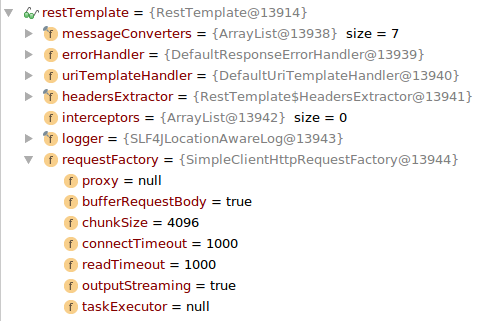
\includegraphics[scale=0.6]{resttempldatedefaulttimeout.png}
	\caption{RestTemplate默认超时时间}
	\label{fig:resttempldatedefaulttimeout}
\end{figure}

上图是Debug跟踪时查看的RestTemplate默认变量。由图中可以看出,默认超时时间是1秒。此时需要增大Read time out的默认超时时间。自定义超时时间如下代码片段所示:

\begin{lstlisting}[language=Java]
@Bean(name = "commonRestTemplate")
public RestTemplate restTemplate(RestTemplateBuilder restTemplateBuilder) {
	return restTemplateBuilder.setConnectTimeout(5000)
			.setReadTimeout(20000)
			.build();
}
\end{lstlisting}



\subsection{自动化部署(Auto Deploy)}

调动Maven打包命令:


构建后,将文件拷贝到服务器:

\begin{lstlisting}[language=Bash]
#!/usr/bin/env bash

# 当使用未初始化的变量时,程序自动退出
set -u

# 当任何一行命令执行失败时,自动退出脚本
set -e

# 在运行结果之前,先输出执行的那一行命令
set -x

readonly APP_ID=""
readonly APP_KEY=""
readonly PROJECT_DIR="/var/lib/jenkins/workspace/web-ci-59"
readonly BUILD_OUTPUT_DIR="/var/lib/jenkins/workspace/web-ci-59/cms/target"

BUILD_DIST_FILENAME=${BUILD_OUTPUT_DIR}/cms.war

cd ${BUILD_OUTPUT_DIR}

#
# 文件过大,无法拷贝
# 将大文件拆分
#
split -b 80M ${BUILD_DIST_FILENAME}

CURRENT_TIME=`date '+%Y-%m-%d %H:%M:%S'`

CONST_STR="ysf"

#
# 生成TOKEN
# 接口各项认证参数的排列顺序是:
# 时间戳(timestamp)、AppKey、随机字符串(echostr)
#
TOKEN=`echo -n ${APP_ID}${APP_KEY}${CURRENT_TIME}${CONST_STR}|md5sum|awk '{print $1}'`
SEQUENCE_TOKEN=`echo -n ${CURRENT_TIME}${APP_ID}${APP_KEY}${CONST_STR}|shasum -a 1|awk '{print $1}'`


# 请求服务端,上传主文件
COMMAND=`curl -H "APPID:$APP_ID" \
-H "TIMESTAMP:$CURRENT_TIME" \
-H "ECHOSTR:$CONST_STR" \
-H "TOKEN:$SEQUENCE_TOKEN" \
-F "file=@${BUILD_OUTPUT_DIR}/xaa" \
http://192.168.1.11:8083/api/fileExchange/upload`

COMMAND=`curl -H "APPID:$APP_ID" \
-H "TIMESTAMP:$CURRENT_TIME" \
-H "ECHOSTR:$CONST_STR" \
-H "TOKEN:$SEQUENCE_TOKEN" \
-F "file=@${BUILD_OUTPUT_DIR}/xab" \
http://192.168.1.11:8083/api/fileExchange/upload`
\end{lstlisting}

在上传文件时,由于限制了文件大小(估计是100MB),当部署文件大于100MB时,使用split命令,拆分成多个小文件分开上传,上传后通过cat命令组装成war包,组装后的文件与原始文件一致,可以通过对比文件的MD5值来判断。

\subsection{无法获取数据库连接}

最近2天网站运行一段时间后会突然宕掉,日志输出无法获取数据库连接(Could not get JDBC connection),初步推测是数据库连接泄漏,造成数据库可用连接被使用完,主备节点都拿不到连接,造成此问题,目前连接由连接池进行管理,一般情况下是不需要人工干预数据库的连接申请和释放,也有可能是某处进行了手工申请数据库连接。定时检测连接池数量:

\begin{lstlisting}[language=Bash]
# 每5秒查看一次到数据库连接个数
nohup watch -n 5 'lsof -i:5236|wc -l >> pool.log'
\end{lstlisting}

经过观察,数据库连接稳定在300-310之间,暂时还无法断定是连接池泄漏导致。



解决的方式:

\begin{itemize}
	\item{增大数据库Session数量}
	\item{安装新的数据库,将部分数据连接转移到新库}
\end{itemize}




\begin{thebibliography}{0}
\bibitem{蒋金楠MVC框架揭秘}
蒋金楠.《ASP.NET MVC 5框架揭秘》.电子工业出版社,2014.
\end{thebibliography}

%\bibitem{BSD}
%B. Birch, H. P. F. Swinnerton-Dyer, \emph{Notes on ellptic curves (II)}. J Reine Angrew Math, 1965, 218:79-108.
\end{document}
